\chapter{Lecture 2: String Theory and M-Theory}

These notes follow Leonard Susskind's second lecture on string theory, curated in this archive by LazyingArt LLC. The lecture begins by putting the needed mathematics on the board before it becomes a nuisance later: discrete approximations on an interval, boundary conditions, Fourier expansions, orthogonality, and the harmonic oscillator. Only after that stockpile is in place does the lecture turn to the physical questions: when a string may count as a particle, how the infinite-momentum or light-front viewpoint converts the problem into an exact two-dimensional mechanical system, why the endpoint condition must be Neumann, and how the open string decomposes into an infinite collection of uncoupled oscillators.

\section{Mathematical Preliminaries on the Interval $[0,\pi]$}

Susskind begins in a deliberately preparatory mood. We are not yet doing string dynamics; we are putting on the board the interval calculus that will later let us pass smoothly from a chain of masses to a continuum string.

Take first a function \(x(\sigma)\) on the interval \(0\leq \sigma \leq \pi\). We discretize the interval into \(N\) equal pieces, write \(\Delta \sigma=\pi/N\), and replace the continuous function by sampled values \(x_i\). Then the standard calculus replacements are
\begin{align}
x(\sigma) &\longrightarrow x_i, \\
\Delta x_i \equiv x_i-x_{i-1} &\approx \frac{\partial x}{\partial \sigma}\,\Delta \sigma, \\
\sum_i x_i\,\Delta \sigma &\longrightarrow \int_0^\pi x(\sigma)\,d\sigma .
\end{align}
Nothing deep is being claimed here. The point is simply that these are the rules we will use again, almost immediately, for the string itself.

The next piece of structure concerns the behavior at the endpoints. Two classes of functions are distinguished.

\paragraph{Dirichlet boundary conditions.}
These are the functions pinned at the ends:
\begin{equation}
x(0)=x(\pi)=0.
\end{equation}
A violin string with fixed endpoints is the standard picture.

\paragraph{Neumann boundary conditions.}
These are the functions flat at the ends:
\begin{equation}
\left.\frac{\partial x}{\partial \sigma}\right|_{\sigma=0}
=
\left.\frac{\partial x}{\partial \sigma}\right|_{\sigma=\pi}
=0.
\end{equation}
The function need not vanish there, but its slope does.

Once the boundary condition is fixed, the appropriate Fourier basis is fixed with it. On the interval \([0,\pi]\) we write
\begin{align}
x_D(\sigma) &= \sum_{n=1}^{\infty} x_n \sin n\sigma, \\
x_N(\sigma) &= \sum_{n=0}^{\infty} x_n \cos n\sigma .
\end{align}
The lecture stresses a simple but important fact: differentiation swaps the two classes. Differentiate a Dirichlet function and one gets a Neumann function; differentiate a Neumann function and one gets a Dirichlet function.

To use these expansions effectively we also need the orthogonality relations. In the form needed later,
\begin{align}
\int_0^\pi \cos n\sigma \cos m\sigma\,d\sigma &= 0 \qquad (n\neq m), \\
\int_0^\pi \cos^2 n\sigma\,d\sigma &= \frac{\pi}{2} \qquad (n\geq 1), \\
\int_0^\pi d\sigma &= \pi, \\
\int_0^\pi \sin n\sigma \sin m\sigma\,d\sigma &= \frac{\pi}{2}\delta_{nm} \qquad (n,m\geq 1).
\end{align}

\begin{remark}
The transcript is garbled near the special \(n=0\) cosine mode, but the intended completion is clearly the standard one above: the zero cosine mode is exceptional because \(\cos 0\sigma=1\).
\end{remark}

Finally, Susskind reminds us of the normalized harmonic oscillator. After rescaling so that the mass is one, the energy and Lagrangian are
\begin{equation}
E_{\mathrm{osc}}=\frac{1}{2}\dot x^{\,2}+\frac{1}{2}\omega^2 x^2,
\qquad
L_{\mathrm{osc}}=\frac{1}{2}\dot x^{\,2}-\frac{1}{2}\omega^2 x^2.
\end{equation}
The quantum oscillator will return later, but already one fact is worth storing: its levels are separated by units of \(\omega\), up to the familiar ground-state offset that Susskind does not yet want to emphasize.

\section{What Makes a String a Particle?}

With the mathematical tools in place, the lecture inserts a conceptual obstacle that should not be skipped. A string, as it is about to be modeled, is plainly made of many pieces. In what sense, then, can we call it a particle at all?

The answer is not that particles must be pointlike. The lecture goes out of its way to reject that. Electrons are surrounded by virtual clouds; protons are composite; even photons are not to be thought of here as featureless geometric points. Pointlikeness is not the criterion.

The real contrast is between a system whose low-lying states are isolated and a system whose nearby excitations are so densely packed that the object behaves like continuum matter. A cup of coffee has a position and a mass, but it also has an enormous number of neighboring states separated by tiny energies. Stir it slightly, excite a sound mode, disturb one molecule, and one moves almost continuously through nearby states. That is not how a particle behaves.

\subsection{Question \& Answer}

\paragraph{Question.}
When does a composite object count as a particle rather than ``mush''?

\paragraph{Answer.}
A composite object counts as a particle when its excitation spectrum has appreciable gaps above the ground state. If the first few excited states lie well above the lowest one, the object behaves as an isolated quantum species. If instead there are innumerable states at arbitrarily tiny energy separations, the object behaves like matter with effectively continuous internal excitations.

This is why a proton still counts as a particle: its excited states are there, but not infinitesimally close. And this is why an ordinary violin string does not count as a particle: compared with its total mass, the vibrational excitations cost almost nothing. For the strings of string theory, by contrast, the relevant gap is taken to be enormous, of order the Planck scale. That is the sense in which a quantum string may still behave as a particle.

\section{Review of the Infinite-Momentum / Light-Front Trick}

The lecture now returns to the viewpoint introduced previously. The goal is to describe a highly relativistic extended object by an exactly nonrelativistic-looking transverse dynamics.

Start with a system of relativistic mass \(M\), boosted hard in the \(z\)-direction. Its energy is
\begin{equation}
E=\sqrt{P_z^2+p_x^2+p_y^2+M^2}.
\end{equation}
When \(P_z\) is much larger than the transverse momenta and much larger than \(M\), we expand:
\begin{equation}
E \approx P_z+\frac{p_x^2+p_y^2+M^2}{2P_z}.
\end{equation}
The first term is kinematically trivial for the questions at hand. It depends only on the conserved longitudinal momentum and not on the internal state, so we subtract it and write
\begin{equation}
E-P_z=\frac{p_x^2+p_y^2+M^2}{2P_z}.
\end{equation}

Now comes the interpretive move that matters most in this review. Energy is Hamiltonian; Hamiltonian controls time evolution. If we keep the ordinary time variable while boosting \(P_z\) to be very large, the internal motion slows by time dilation and the right-hand side tends to zero. The remedy is not to discard the internal dynamics, but to rescale time so that we follow the slow internal clock of the boosted system. Equivalently, one multiplies by the same large factor \(P_z\). Up to the common overall normalization, the limiting Hamiltonian becomes
\begin{equation}
P_z(E-P_z)=\frac{1}{2}\left(p_x^2+p_y^2+M^2\right).
\end{equation}
This has exactly the look of a two-dimensional nonrelativistic Hamiltonian. The transverse motion is described by quadratic momenta, while the quantity ordinarily called rest energy is encoded here through \(M^2\), not \(M\) itself.

\begin{figure}[htbp]
\centering

\includegraphics[width=0.72\textwidth]{lecture_02_figure_02.png}
\caption{Hamiltonian form of the boosted energy. The board line beginning with \(H=\) marks the shift from a kinematic expansion to a Hamiltonian interpretation.}
\label{fig:lecture02-lightfront}
\end{figure}

\begin{remark}
Susskind briefly objects to the phrase ``light cone'' here and prefers ``light front.'' The point of the lecture is not terminological. What matters is the structural fact: after the boost and the time rescaling, the transverse dynamics are exactly nonrelativistic in form.
\end{remark}

This is the license for everything that follows. A string, viewed in this way, may be treated as a mechanical system moving in two transverse directions, which we now call \(X\) and \(Y\).

\section{A String as Mass Points and Springs}

We now turn fully to the string itself. The open string is modeled as \(N\) mass points joined by \(N-1\) springs. The label \(\sigma\) runs from \(0\) to \(\pi\). This is only a convention, but a useful one: the interval \([0,\pi]\) is reserved for an open string with endpoints, while \(0\leq \sigma <2\pi\) will later be used for a closed string.

The discrete transverse energy is
\begin{equation}
E=\sum_i\left[
\frac{\mu}{2}\bigl(\dot X_i^2+\dot Y_i^2\bigr)
+
\frac{k}{2}\bigl((\Delta X_i)^2+(\Delta Y_i)^2\bigr)
\right].
\end{equation}
The lecture board at this stage writes the bead mass as \(m\), but it is better to rename it \(\mu\) so that it is not confused with the relativistic mass of the string state.

\begin{figure}[htbp]
\centering

\includegraphics[width=0.72\textwidth]{lecture_02_figure_03.png}
\caption{Discrete string as mass points and springs. The lecture pairs the bead-chain sketch directly with the discrete energy formula.}
\label{fig:lecture02-discrete-board}
\end{figure}

\begin{figure}[htbp]
\centering
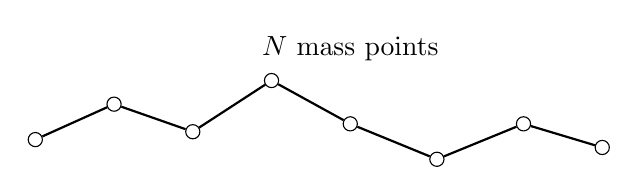
\begin{tikzpicture}[scale=1.0]
\draw[thick] (0,0) -- (1.0,0.45) -- (2.0,0.10) -- (3.0,0.75) -- (4.0,0.20) -- (5.1,-0.25) -- (6.2,0.20) -- (7.2,-0.10);
\foreach \x/\y in {0/0,1.0/0.45,2.0/0.10,3.0/0.75,4.0/0.20,5.1/-0.25,6.2/0.20,7.2/-0.10}
{
  \filldraw[white] (\x,\y) circle (0.09);
  \draw (\x,\y) circle (0.09);
}
\node at (4.0,1.15) {$N$ mass points};
\end{tikzpicture}
\caption{A clean redraw of the bead-chain model used to take the continuum limit.}
\label{fig:lecture02-discrete-tikz}
\end{figure}

The next question is how these parameters must scale as \(N\to\infty\). The total analog mass of the string should remain fixed, so each bead mass must scale like
\begin{equation}
\mu=\frac{1}{N}.
\end{equation}
Likewise, the individual springs must become stiffer as we subdivide the string more finely. Springs in series make the whole string easier to stretch, so to keep the macroscopic stiffness fixed the microscopic spring constant must grow with \(N\). Susskind chooses
\begin{equation}
k=\frac{N}{\pi^2},
\end{equation}
with the factor of \(\pi^2\) inserted only to simplify later formulas.

At this point the lecture has done something characteristic: it has not postulated a continuum action out of thin air. It has built the continuum string from a discrete chain and chosen the scalings that keep the limit nontrivial.

\section{Continuum Energy, Lagrangian, and Wave Interpretation}

Now we cash in the preliminary calculus formulas. Since \(\Delta \sigma=\pi/N\), we may rewrite the discrete sums as integrals.

\paragraph{A worked passage from the discrete chain to the continuum.}
For the \(X\)-sector kinetic term,
\begin{align}
\sum_i \frac{\mu}{2}\dot X_i^2
&=
\sum_i \frac{1}{2N}\dot X_i^2 \\
&=
\frac{1}{2\pi}\sum_i \dot X_i^2\,\Delta \sigma \\
&\longrightarrow
\frac{1}{2\pi}\int_0^\pi d\sigma
\left(\frac{\partial X}{\partial \tau}\right)^2 .
\end{align}
For the spring term we use \(\Delta X_i\approx (\partial_\sigma X)\Delta \sigma\):
\begin{align}
\sum_i \frac{k}{2}(\Delta X_i)^2
&\approx
\sum_i \frac{N}{2\pi^2}
\left(\frac{\partial X}{\partial \sigma}\right)^2
(\Delta \sigma)^2 \\
&=
\sum_i \frac{1}{2N}
\left(\frac{\partial X}{\partial \sigma}\right)^2 \\
&=
\frac{1}{2\pi}\sum_i
\left(\frac{\partial X}{\partial \sigma}\right)^2\Delta \sigma \\
&\longrightarrow
\frac{1}{2\pi}\int_0^\pi d\sigma
\left(\frac{\partial X}{\partial \sigma}\right)^2 .
\end{align}
The same derivation applies to \(Y\).

Thus the continuum Lagrangian takes the form
\begin{equation}
L=
\frac{1}{2\pi}\int_0^\pi d\sigma
\left[
\left(\frac{\partial X}{\partial \tau}\right)^2
+
\left(\frac{\partial Y}{\partial \tau}\right)^2
-
\left(\frac{\partial X}{\partial \sigma}\right)^2
-
\left(\frac{\partial Y}{\partial \sigma}\right)^2
\right].
\end{equation}
The corresponding energy differs only by changing the minus signs in the spatial derivative terms to plus signs.

\begin{figure}[htbp]
\centering

\includegraphics[width=0.76\textwidth]{lecture_02_figure_04.png}
\caption{Continuum string Lagrangian. The board catches the moment when the potential term enters with the crucial minus sign.}
\label{fig:lecture02-continuum}
\end{figure}

We should also keep the wave interpretation because the lecture does. If one thinks of \(\sigma\) as a spatial coordinate on a line and \(X(\sigma,\tau)\) as a field, this is exactly the energy of a simple wave system. Disturbances move left and right along the interval and reflect at the endpoints. Under Dirichlet reflection the wave flips sign; under Neumann reflection it reflects without such inversion. Susskind remarks that one could write the wave equation by varying this Lagrangian, but the lecture does not need it, so we should resist the urge to do more than that.

A final notational point is made here. The time variable \(\tau\) is the rescaled time appropriate to the boosted description; Susskind loosely calls it proper time. For the present nonrelativistic-looking transverse problem, we may simply treat \(\tau\) as the time variable with respect to which the string wiggles.

\section{Endpoint Dynamics and the Boundary-Condition Puzzle}

At this stage the lecture raises its first sharp local puzzle. We have a continuum string on an interval, but what boundary condition should its endpoints satisfy? The opening mathematical discussion has displayed both Dirichlet and Neumann possibilities. Why should the open string choose one rather than the other?

\begin{figure}[htbp]
\centering

\includegraphics[width=0.68\textwidth]{lecture_02_figure_05.png}
\caption{Discrete difference becomes derivative times spacing. This local replacement is the key step in the endpoint-force argument.}
\label{fig:lecture02-endpoint-board}
\end{figure}

\begin{figure}[htbp]
\centering
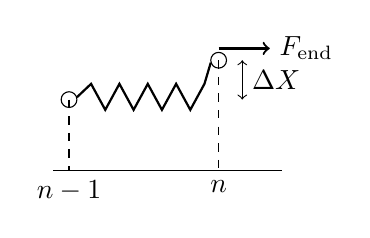
\begin{tikzpicture}[scale=1.0]
\draw[thin] (-0.2,-0.8) -- (2.7,-0.8);
\filldraw[white] (0,0.10) circle (0.10);
\draw (0,0.10) circle (0.10);
\filldraw[white] (1.9,0.60) circle (0.10);
\draw (1.9,0.60) circle (0.10);
\draw[thick]
(0.10,0.13) -- (0.28,0.30) -- (0.46,-0.03) -- (0.64,0.30) -- (0.82,-0.03) -- (1.00,0.30) -- (1.18,-0.03) -- (1.36,0.30) -- (1.54,-0.03) -- (1.72,0.30) -- (1.80,0.57);
\draw[dashed] (0,0.10) -- (0,-0.8);
\draw[dashed] (1.9,0.60) -- (1.9,-0.8);
\node[below] at (0,-0.8) {$n-1$};
\node[below] at (1.9,-0.8) {$n$};
\draw[<->] (2.2,0.10) -- (2.2,0.60);
\node[right] at (2.2,0.35) {$\Delta X$};
\draw[->,thick] (1.9,0.75) -- (2.55,0.75);
\node[right] at (2.55,0.75) {$F_{\mathrm{end}}$};
\end{tikzpicture}
\caption{Endpoint geometry for the Newton-law argument. The last mass point feels a force from only one spring.}
\label{fig:lecture02-endpoint-tikz}
\end{figure}

\subsection{Question \& Answer}

\paragraph{Question.}
Why must the open-string endpoint satisfy Neumann rather than Dirichlet boundary conditions?

\paragraph{Answer.}
Because the endpoint is special: unlike an interior mass point, it is pulled only from one side. Newton's law at that endpoint then forces the slope of the string to vanish in the continuum limit.

Here is the argument in the form the lecture uses. Let the last bead be labeled \(n\), with the penultimate bead \(n-1\). Hooke's law gives the endpoint force
\begin{equation}
F_{\mathrm{end}}\sim k\,\Delta X .
\end{equation}
Now replace the discrete difference by its continuum form,
\begin{equation}
\Delta X=\frac{\partial X}{\partial \sigma}\,\Delta \sigma .
\end{equation}
Since \(k\sim N\) while \(\Delta \sigma\sim 1/N\), the factors of \(N\) cancel and one finds
\begin{equation}
F_{\mathrm{end}} \propto \frac{\partial X}{\partial \sigma}.
\end{equation}
But Newton's law still applies to the endpoint mass:
\begin{equation}
F_{\mathrm{end}}=\mu\,\frac{\partial^2 X}{\partial \tau^2},
\qquad
\mu\sim \frac{1}{N}.
\end{equation}
Therefore, unless \(\partial_\sigma X\) vanishes at the endpoint, the acceleration \(\partial_\tau^2 X\) grows like \(N\) and becomes infinite as the continuum limit is taken. That is physically unacceptable. The cure is
\begin{equation}
\left.\frac{\partial X}{\partial \sigma}\right|_{\sigma=0,\pi}=0.
\end{equation}
The same argument applies to \(Y\). Thus the free open-string endpoint obeys Neumann boundary conditions.

This is exactly the sort of moment the lecture wants us to notice. Neumann conditions are not inserted by aesthetic taste; they are forced by the endpoint dynamics.

\section{Fourier Modes, Harmonic Oscillators, and the First Quantum Spectrum}

With the classical system finally specified, the lecture turns to quantization. The first move is again mathematical: expand the Neumann string in cosine modes,
\begin{equation}
X(\sigma,\tau)=\sum_{n=0}^{\infty} X_n(\tau)\cos n\sigma,
\qquad
Y(\sigma,\tau)=\sum_{n=0}^{\infty} Y_n(\tau)\cos n\sigma.
\end{equation}
The time dependence sits entirely in the coefficients \(X_n(\tau)\) and \(Y_n(\tau)\). This is the natural place for the string to wiggle.

Differentiating with respect to \(\sigma\) gives
\begin{equation}
\frac{\partial X}{\partial \sigma}
=
-\sum_{n=1}^{\infty} n\,X_n(\tau)\sin n\sigma .
\end{equation}
The lecture board momentarily suggests a sum beginning at \(n=0\), but the cleaned formula must start at \(n=1\), since the differentiated zero mode vanishes.

\begin{figure}[htbp]
\centering

\includegraphics[width=0.70\textwidth]{lecture_02_figure_06.png}
\caption{Mode expansion of the \(\sigma\)-derivative. The crucial board content is the minus sign, the factor of \(n\), and the passage from cosines to sines.}
\label{fig:lecture02-modes}
\end{figure}

Now insert the mode expansion into the energy. Orthogonality kills all cross-terms with \(n\neq m\), so the double sums collapse to single sums. The zero mode must be handled separately because
\(\int_0^\pi d\sigma=\pi\), not \(\pi/2\).

For the \(X\)-sector one finds
\begin{equation}
E_X=
\frac{1}{2}\dot X_0^{\,2}
+
\frac{1}{4}\sum_{n=1}^{\infty}
\left(
\dot X_n^{\,2}+n^2X_n^{\,2}
\right),
\end{equation}
and similarly
\begin{equation}
E_Y=
\frac{1}{2}\dot Y_0^{\,2}
+
\frac{1}{4}\sum_{n=1}^{\infty}
\left(
\dot Y_n^{\,2}+n^2Y_n^{\,2}
\right).
\end{equation}
Hence the full internal vibrational energy is
\begin{equation}
E_{\mathrm{int}}
=
\frac{1}{4}\sum_{n=1}^{\infty}
\left(
\dot X_n^{\,2}+n^2X_n^{\,2}
+
\dot Y_n^{\,2}+n^2Y_n^{\,2}
\right).
\end{equation}

The interpretation is immediate. The zero modes \(X_0\) and \(Y_0\) are just center-of-mass motion. They have no restoring force, hence no oscillator frequency. Every nonzero mode, by contrast, is a harmonic oscillator, and the \(n\)-th one has frequency
\begin{equation}
\omega_n=n,
\qquad
n\geq 1.
\end{equation}
So the open string is not a single oscillator but a doubly infinite tower of them: one \(X\)-oscillator and one \(Y\)-oscillator for each harmonic \(n\geq 1\).

Up to the same overall light-front normalization fixed earlier, this internal energy is what becomes the relativistic mass squared of the string state. That is the decisive bridge between the mode expansion and particle physics.

Quantization is now straightforward. For the \(n\)-th oscillator, if \(Q_n\) quanta are present and \(\hbar=1\), the excitation energy above the ground-state offset is
\begin{equation}
\Delta E_n = Q_n\,\omega_n = Q_n\,n.
\end{equation}
Susskind does not want to pin down the absolute ground-state energy yet, so we keep it unspecified.

The first few levels are easy to organize.

\paragraph{Ground state.}
All oscillators are unexcited. This is not empty space; it is a single open string in its lowest state.

\paragraph{First excited level.}
Excite the \(n=1\) oscillator once. One may do this in the \(X\)-direction or in the \(Y\)-direction, so the first excited level has multiplicity \(2\).

\paragraph{Second excited level.}
Now the total excitation energy is \(2\). There are five possibilities:
\begin{itemize}
\item two quanta in the \(n=1\) \(X\)-oscillator,
\item two quanta in the \(n=1\) \(Y\)-oscillator,
\item one quantum in each of the \(n=1\) \(X\)- and \(Y\)-oscillators,
\item one quantum in the \(n=2\) \(X\)-oscillator,
\item one quantum in the \(n=2\) \(Y\)-oscillator.
\end{itemize}
Thus the second excited level has multiplicity \(5\).

This is the payoff of the earlier philosophical detour. The open string has a discrete spectrum with genuine gaps. It is therefore particle-like in precisely the sense the lecture wanted to make sharp.

The lecture closes by pointing outward. Open strings can join and split. Once such interactions are admitted, a fluctuating open string can bring one endpoint into contact with another endpoint and thereby produce a closed string. So one may have a theory of closed strings without open strings, but not a theory of open strings without closed strings. As a rough preview only: open-string states often behave like photons, while closed-string states behave like gravitons.

\section{Summary}

The lecture has taken a very controlled path. First it stocked the board with the mathematics of functions on \([0,\pi]\): discretization, boundary conditions, Fourier modes, orthogonality, and the harmonic oscillator. Then it sharpened the meaning of a particle by appealing to spectral gaps rather than pointlikeness. With that in hand, the infinite-momentum or light-front trick recast the relativistic string as an exact two-dimensional mechanical system. The open string emerged first as a chain of beads and springs, then as a continuum field with Neumann boundary conditions forced by endpoint dynamics, and finally as an infinite collection of uncoupled harmonic oscillators. The result is the first quantum spectrum of the open string, already discrete enough to justify the central claim: a string can indeed behave like a particle.